% Created by tikzDevice version 0.12.6 on 2026-11-04 18:16:13
% !TEX encoding = UTF-8 Unicode
\documentclass[tikz,border=0pt]{standalone}\usepackage{tikz}
\usetikzlibrary{calc}
\usepackage[T1]{fontenc}
\usepackage[sc]{mathpazo}
\usepackage{amsmath}\begin{document}

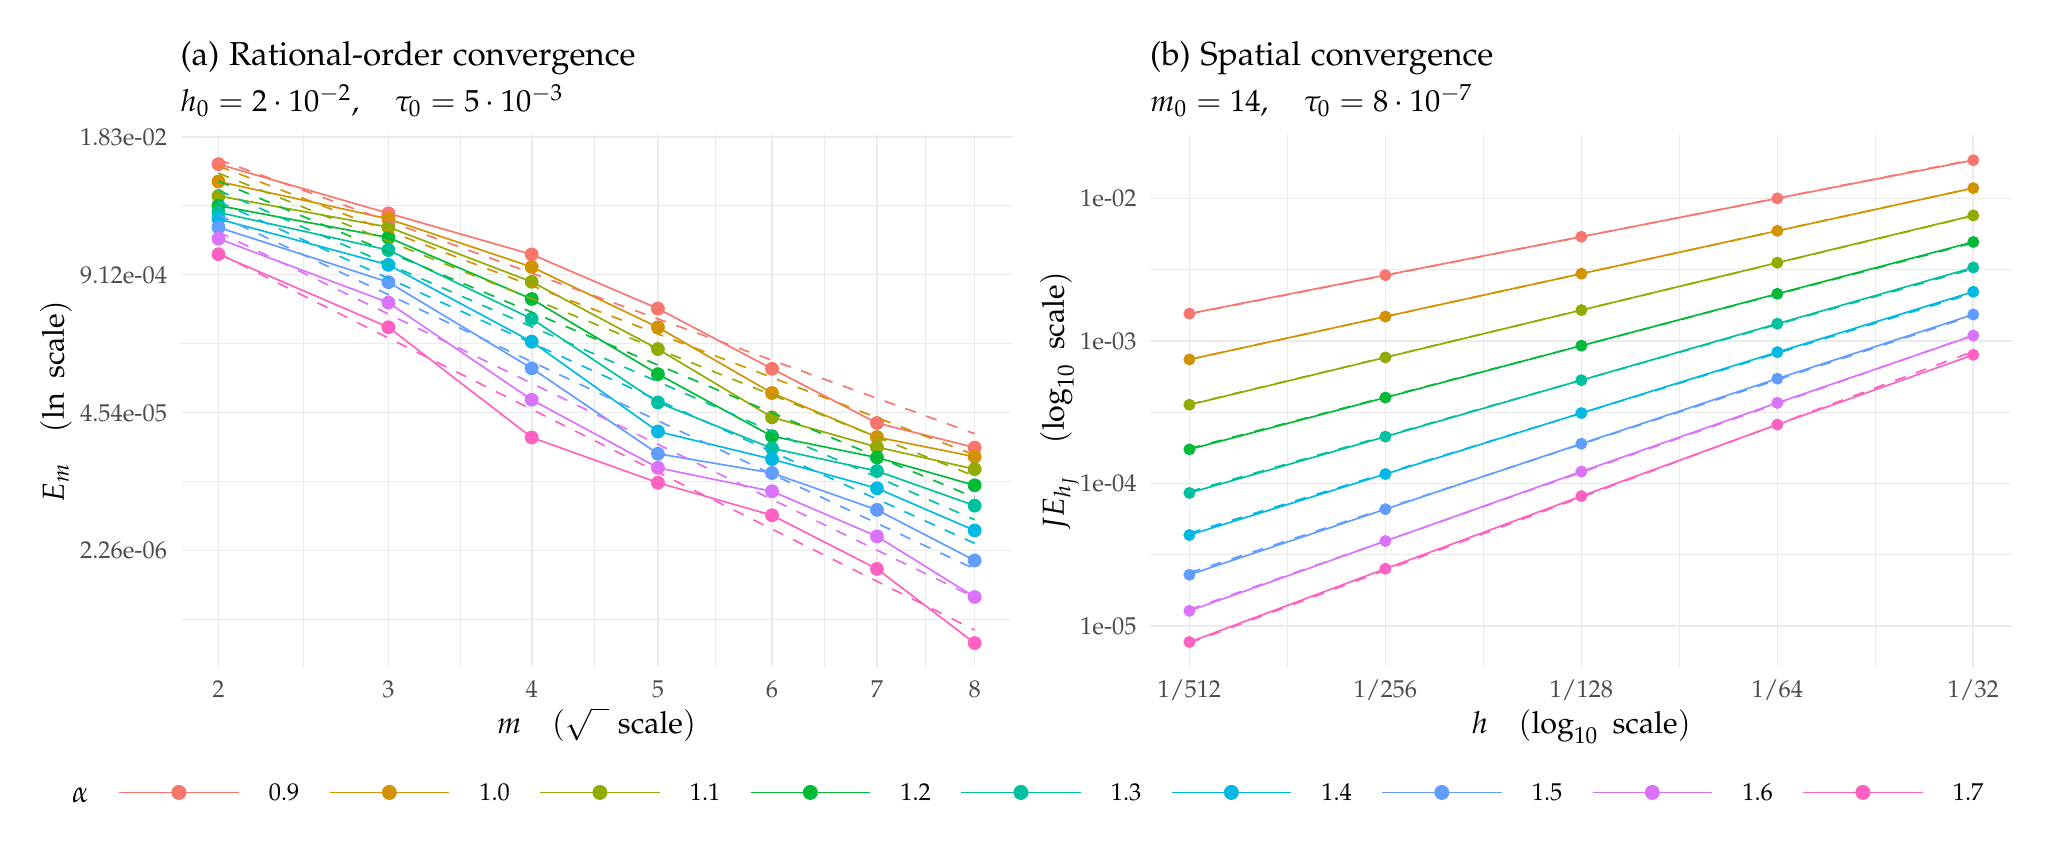
\begin{tikzpicture}[x=1pt,y=1pt]
\definecolor{fillColor}{RGB}{255,255,255}
\path[use as bounding box,fill=fillColor,fill opacity=0.00] (0,0) rectangle (722.70,289.08);
\begin{scope}
\path[clip] (  0.00, 25.45) rectangle (361.35,289.08);
\definecolor{fillColor}{RGB}{255,255,255}

\path[fill=fillColor] (  0.00, 25.45) rectangle (361.35,289.08);
\end{scope}
\begin{scope}
\path[clip] ( 55.28, 57.98) rectangle (355.85,250.13);
\definecolor{drawColor}{gray}{0.92}

\path[draw=drawColor,line width= 0.3pt,line join=round] ( 55.28, 75.24) --
	(355.85, 75.24);

\path[draw=drawColor,line width= 0.3pt,line join=round] ( 55.28,125.08) --
	(355.85,125.08);

\path[draw=drawColor,line width= 0.3pt,line join=round] ( 55.28,174.92) --
	(355.85,174.92);

\path[draw=drawColor,line width= 0.3pt,line join=round] ( 55.28,224.76) --
	(355.85,224.76);

\path[draw=drawColor,line width= 0.3pt,line join=round] ( 99.65, 57.98) --
	( 99.65,250.13);

\path[draw=drawColor,line width= 0.3pt,line join=round] (156.24, 57.98) --
	(156.24,250.13);

\path[draw=drawColor,line width= 0.3pt,line join=round] (204.93, 57.98) --
	(204.93,250.13);

\path[draw=drawColor,line width= 0.3pt,line join=round] (248.35, 57.98) --
	(248.35,250.13);

\path[draw=drawColor,line width= 0.3pt,line join=round] (287.93, 57.98) --
	(287.93,250.13);

\path[draw=drawColor,line width= 0.3pt,line join=round] (324.54, 57.98) --
	(324.54,250.13);

\path[draw=drawColor,line width= 0.6pt,line join=round] ( 55.28,100.16) --
	(355.85,100.16);

\path[draw=drawColor,line width= 0.6pt,line join=round] ( 55.28,150.00) --
	(355.85,150.00);

\path[draw=drawColor,line width= 0.6pt,line join=round] ( 55.28,199.84) --
	(355.85,199.84);

\path[draw=drawColor,line width= 0.6pt,line join=round] ( 55.28,249.68) --
	(355.85,249.68);

\path[draw=drawColor,line width= 0.6pt,line join=round] ( 68.94, 57.98) --
	( 68.94,250.13);

\path[draw=drawColor,line width= 0.6pt,line join=round] (130.35, 57.98) --
	(130.35,250.13);

\path[draw=drawColor,line width= 0.6pt,line join=round] (182.13, 57.98) --
	(182.13,250.13);

\path[draw=drawColor,line width= 0.6pt,line join=round] (227.74, 57.98) --
	(227.74,250.13);

\path[draw=drawColor,line width= 0.6pt,line join=round] (268.97, 57.98) --
	(268.97,250.13);

\path[draw=drawColor,line width= 0.6pt,line join=round] (306.89, 57.98) --
	(306.89,250.13);

\path[draw=drawColor,line width= 0.6pt,line join=round] (342.19, 57.98) --
	(342.19,250.13);
\definecolor{drawColor}{RGB}{248,118,109}

\path[draw=drawColor,line width= 0.6pt,line join=round] ( 68.94,239.77) --
	(130.35,221.99) --
	(182.13,207.14) --
	(227.74,187.57) --
	(268.97,165.81) --
	(306.89,146.22) --
	(342.19,137.35);
\definecolor{drawColor}{RGB}{211,146,0}

\path[draw=drawColor,line width= 0.6pt,line join=round] ( 68.94,233.48) --
	(130.35,219.97) --
	(182.13,202.61) --
	(227.74,180.79) --
	(268.97,157.05) --
	(306.89,141.12) --
	(342.19,134.03);
\definecolor{drawColor}{RGB}{147,170,0}

\path[draw=drawColor,line width= 0.6pt,line join=round] ( 68.94,228.27) --
	(130.35,217.01) --
	(182.13,197.24) --
	(227.74,172.94) --
	(268.97,148.28) --
	(306.89,137.52) --
	(342.19,129.56);
\definecolor{drawColor}{RGB}{0,186,56}

\path[draw=drawColor,line width= 0.6pt,line join=round] ( 68.94,224.77) --
	(130.35,213.24) --
	(182.13,191.02) --
	(227.74,163.89) --
	(268.97,141.45) --
	(306.89,133.74) --
	(342.19,123.71);
\definecolor{drawColor}{RGB}{0,193,159}

\path[draw=drawColor,line width= 0.6pt,line join=round] ( 68.94,222.35) --
	(130.35,208.71) --
	(182.13,183.87) --
	(227.74,153.65) --
	(268.97,137.07) --
	(306.89,128.89) --
	(342.19,116.37);
\definecolor{drawColor}{RGB}{0,185,227}

\path[draw=drawColor,line width= 0.6pt,line join=round] ( 68.94,219.95) --
	(130.35,203.37) --
	(182.13,175.61) --
	(227.74,143.15) --
	(268.97,133.15) --
	(306.89,122.63) --
	(342.19,107.40);
\definecolor{drawColor}{RGB}{97,156,255}

\path[draw=drawColor,line width= 0.6pt,line join=round] ( 68.94,216.90) --
	(130.35,197.12) --
	(182.13,165.99) --
	(227.74,135.11) --
	(268.97,128.16) --
	(306.89,114.83) --
	(342.19, 96.56);
\definecolor{drawColor}{RGB}{219,114,251}

\path[draw=drawColor,line width= 0.6pt,line join=round] ( 68.94,212.80) --
	(130.35,189.73) --
	(182.13,154.63) --
	(227.74,130.03) --
	(268.97,121.54) --
	(306.89,105.26) --
	(342.19, 83.35);
\definecolor{drawColor}{RGB}{255,97,195}

\path[draw=drawColor,line width= 0.6pt,line join=round] ( 68.94,207.21) --
	(130.35,180.82) --
	(182.13,141.00) --
	(227.74,124.65) --
	(268.97,112.89) --
	(306.89, 93.50) --
	(342.19, 66.71);
\definecolor{fillColor}{RGB}{248,118,109}

\path[fill=fillColor] ( 68.94,239.77) circle (  2.50);

\path[fill=fillColor] (130.35,221.99) circle (  2.50);

\path[fill=fillColor] (182.13,207.14) circle (  2.50);

\path[fill=fillColor] (227.74,187.57) circle (  2.50);

\path[fill=fillColor] (268.97,165.81) circle (  2.50);

\path[fill=fillColor] (306.89,146.22) circle (  2.50);

\path[fill=fillColor] (342.19,137.35) circle (  2.50);
\definecolor{fillColor}{RGB}{211,146,0}

\path[fill=fillColor] ( 68.94,233.48) circle (  2.50);

\path[fill=fillColor] (130.35,219.97) circle (  2.50);

\path[fill=fillColor] (182.13,202.61) circle (  2.50);

\path[fill=fillColor] (227.74,180.79) circle (  2.50);

\path[fill=fillColor] (268.97,157.05) circle (  2.50);

\path[fill=fillColor] (306.89,141.12) circle (  2.50);

\path[fill=fillColor] (342.19,134.03) circle (  2.50);
\definecolor{fillColor}{RGB}{147,170,0}

\path[fill=fillColor] ( 68.94,228.27) circle (  2.50);

\path[fill=fillColor] (130.35,217.01) circle (  2.50);

\path[fill=fillColor] (182.13,197.24) circle (  2.50);

\path[fill=fillColor] (227.74,172.94) circle (  2.50);

\path[fill=fillColor] (268.97,148.28) circle (  2.50);

\path[fill=fillColor] (306.89,137.52) circle (  2.50);

\path[fill=fillColor] (342.19,129.56) circle (  2.50);
\definecolor{fillColor}{RGB}{0,186,56}

\path[fill=fillColor] ( 68.94,224.77) circle (  2.50);

\path[fill=fillColor] (130.35,213.24) circle (  2.50);

\path[fill=fillColor] (182.13,191.02) circle (  2.50);

\path[fill=fillColor] (227.74,163.89) circle (  2.50);

\path[fill=fillColor] (268.97,141.45) circle (  2.50);

\path[fill=fillColor] (306.89,133.74) circle (  2.50);

\path[fill=fillColor] (342.19,123.71) circle (  2.50);
\definecolor{fillColor}{RGB}{0,193,159}

\path[fill=fillColor] ( 68.94,222.35) circle (  2.50);

\path[fill=fillColor] (130.35,208.71) circle (  2.50);

\path[fill=fillColor] (182.13,183.87) circle (  2.50);

\path[fill=fillColor] (227.74,153.65) circle (  2.50);

\path[fill=fillColor] (268.97,137.07) circle (  2.50);

\path[fill=fillColor] (306.89,128.89) circle (  2.50);

\path[fill=fillColor] (342.19,116.37) circle (  2.50);
\definecolor{fillColor}{RGB}{0,185,227}

\path[fill=fillColor] ( 68.94,219.95) circle (  2.50);

\path[fill=fillColor] (130.35,203.37) circle (  2.50);

\path[fill=fillColor] (182.13,175.61) circle (  2.50);

\path[fill=fillColor] (227.74,143.15) circle (  2.50);

\path[fill=fillColor] (268.97,133.15) circle (  2.50);

\path[fill=fillColor] (306.89,122.63) circle (  2.50);

\path[fill=fillColor] (342.19,107.40) circle (  2.50);
\definecolor{fillColor}{RGB}{97,156,255}

\path[fill=fillColor] ( 68.94,216.90) circle (  2.50);

\path[fill=fillColor] (130.35,197.12) circle (  2.50);

\path[fill=fillColor] (182.13,165.99) circle (  2.50);

\path[fill=fillColor] (227.74,135.11) circle (  2.50);

\path[fill=fillColor] (268.97,128.16) circle (  2.50);

\path[fill=fillColor] (306.89,114.83) circle (  2.50);

\path[fill=fillColor] (342.19, 96.56) circle (  2.50);
\definecolor{fillColor}{RGB}{219,114,251}

\path[fill=fillColor] ( 68.94,212.80) circle (  2.50);

\path[fill=fillColor] (130.35,189.73) circle (  2.50);

\path[fill=fillColor] (182.13,154.63) circle (  2.50);

\path[fill=fillColor] (227.74,130.03) circle (  2.50);

\path[fill=fillColor] (268.97,121.54) circle (  2.50);

\path[fill=fillColor] (306.89,105.26) circle (  2.50);

\path[fill=fillColor] (342.19, 83.35) circle (  2.50);
\definecolor{fillColor}{RGB}{255,97,195}

\path[fill=fillColor] ( 68.94,207.21) circle (  2.50);

\path[fill=fillColor] (130.35,180.82) circle (  2.50);

\path[fill=fillColor] (182.13,141.00) circle (  2.50);

\path[fill=fillColor] (227.74,124.65) circle (  2.50);

\path[fill=fillColor] (268.97,112.89) circle (  2.50);

\path[fill=fillColor] (306.89, 93.50) circle (  2.50);

\path[fill=fillColor] (342.19, 66.71) circle (  2.50);
\definecolor{drawColor}{RGB}{248,118,109}

\path[draw=drawColor,line width= 0.6pt,dash pattern=on 4pt off 4pt ,line join=round] ( 68.94,241.40) --
	(130.35,219.14) --
	(182.13,200.38) --
	(227.74,183.85) --
	(268.97,168.90) --
	(306.89,155.16) --
	(342.19,142.37);
\definecolor{drawColor}{RGB}{211,146,0}

\path[draw=drawColor,line width= 0.6pt,dash pattern=on 4pt off 4pt ,line join=round] ( 68.94,239.07) --
	(130.35,215.61) --
	(182.13,195.83) --
	(227.74,178.41) --
	(268.97,162.66) --
	(306.89,148.17) --
	(342.19,134.69);
\definecolor{drawColor}{RGB}{147,170,0}

\path[draw=drawColor,line width= 0.6pt,dash pattern=on 4pt off 4pt ,line join=round] ( 68.94,236.50) --
	(130.35,211.89) --
	(182.13,191.15) --
	(227.74,172.88) --
	(268.97,156.35) --
	(306.89,141.16) --
	(342.19,127.02);
\definecolor{drawColor}{RGB}{0,186,56}

\path[draw=drawColor,line width= 0.6pt,dash pattern=on 4pt off 4pt ,line join=round] ( 68.94,233.64) --
	(130.35,207.94) --
	(182.13,186.27) --
	(227.74,167.18) --
	(268.97,149.93) --
	(306.89,134.06) --
	(342.19,119.29);
\definecolor{drawColor}{RGB}{0,193,159}

\path[draw=drawColor,line width= 0.6pt,dash pattern=on 4pt off 4pt ,line join=round] ( 68.94,230.31) --
	(130.35,203.56) --
	(182.13,181.01) --
	(227.74,161.14) --
	(268.97,143.18) --
	(306.89,126.66) --
	(342.19,111.29);
\definecolor{drawColor}{RGB}{0,185,227}

\path[draw=drawColor,line width= 0.6pt,dash pattern=on 4pt off 4pt ,line join=round] ( 68.94,226.26) --
	(130.35,198.50) --
	(182.13,175.10) --
	(227.74,154.49) --
	(268.97,135.85) --
	(306.89,118.71) --
	(342.19,102.75);
\definecolor{drawColor}{RGB}{97,156,255}

\path[draw=drawColor,line width= 0.6pt,dash pattern=on 4pt off 4pt ,line join=round] ( 68.94,221.33) --
	(130.35,192.60) --
	(182.13,168.37) --
	(227.74,147.03) --
	(268.97,127.74) --
	(306.89,110.00) --
	(342.19, 93.48);
\definecolor{drawColor}{RGB}{219,114,251}

\path[draw=drawColor,line width= 0.6pt,dash pattern=on 4pt off 4pt ,line join=round] ( 68.94,215.25) --
	(130.35,185.58) --
	(182.13,160.56) --
	(227.74,138.52) --
	(268.97,118.59) --
	(306.89,100.27) --
	(342.19, 83.21);
\definecolor{drawColor}{RGB}{255,97,195}

\path[draw=drawColor,line width= 0.6pt,dash pattern=on 4pt off 4pt ,line join=round] ( 68.94,207.52) --
	(130.35,176.93) --
	(182.13,151.15) --
	(227.74,128.43) --
	(268.97,107.89) --
	(306.89, 89.00) --
	(342.19, 71.42);
\end{scope}
\begin{scope}
\path[clip] (  0.00,  0.00) rectangle (722.70,289.08);
\definecolor{drawColor}{gray}{0.30}

\node[text=drawColor,anchor=base east,inner sep=0pt, outer sep=0pt, scale=  0.88] at ( 50.33, 97.11) {2.26e-06};

\node[text=drawColor,anchor=base east,inner sep=0pt, outer sep=0pt, scale=  0.88] at ( 50.33,146.95) {4.54e-05};

\node[text=drawColor,anchor=base east,inner sep=0pt, outer sep=0pt, scale=  0.88] at ( 50.33,196.79) {9.12e-04};

\node[text=drawColor,anchor=base east,inner sep=0pt, outer sep=0pt, scale=  0.88] at ( 50.33,246.63) {1.83e-02};
\end{scope}
\begin{scope}
\path[clip] (  0.00,  0.00) rectangle (722.70,289.08);
\definecolor{drawColor}{gray}{0.30}

\node[text=drawColor,anchor=base,inner sep=0pt, outer sep=0pt, scale=  0.88] at ( 68.94, 46.93) {2};

\node[text=drawColor,anchor=base,inner sep=0pt, outer sep=0pt, scale=  0.88] at (130.35, 46.93) {3};

\node[text=drawColor,anchor=base,inner sep=0pt, outer sep=0pt, scale=  0.88] at (182.13, 46.93) {4};

\node[text=drawColor,anchor=base,inner sep=0pt, outer sep=0pt, scale=  0.88] at (227.74, 46.93) {5};

\node[text=drawColor,anchor=base,inner sep=0pt, outer sep=0pt, scale=  0.88] at (268.97, 46.93) {6};

\node[text=drawColor,anchor=base,inner sep=0pt, outer sep=0pt, scale=  0.88] at (306.89, 46.93) {7};

\node[text=drawColor,anchor=base,inner sep=0pt, outer sep=0pt, scale=  0.88] at (342.19, 46.93) {8};
\end{scope}
\begin{scope}
\path[clip] (  0.00,  0.00) rectangle (722.70,289.08);
\definecolor{drawColor}{RGB}{0,0,0}

\node[text=drawColor,anchor=base,inner sep=0pt, outer sep=0pt, scale=  1.10] at (205.57, 34.07) {$m\quad(\sqrt{\phantom{x}}\mbox{ scale})$};
\end{scope}
\begin{scope}
\path[clip] (  0.00,  0.00) rectangle (722.70,289.08);
\definecolor{drawColor}{RGB}{0,0,0}

\node[text=drawColor,rotate= 90.00,anchor=base,inner sep=0pt, outer sep=0pt, scale=  1.10] at ( 13.12,154.06) {$E_m\quad(\ln\mbox{ scale})$};
\end{scope}
\begin{scope}
\path[clip] (  0.00,  0.00) rectangle (722.70,289.08);
\definecolor{drawColor}{RGB}{0,0,0}

\node[text=drawColor,anchor=base west,inner sep=0pt, outer sep=0pt, scale=  1.10] at ( 55.28,258.75) {$h_0=2\cdot10^{-2},\quad\tau_0=5\cdot10^{-3}$};
\end{scope}
\begin{scope}
\path[clip] (  0.00,  0.00) rectangle (722.70,289.08);
\definecolor{drawColor}{RGB}{0,0,0}

\node[text=drawColor,anchor=base west,inner sep=0pt, outer sep=0pt, scale=  1.20] at ( 55.28,275.26) {(a) Rational-order convergence};
\end{scope}
\begin{scope}
\path[clip] (361.35, 25.45) rectangle (722.70,289.08);
\definecolor{fillColor}{RGB}{255,255,255}

\path[fill=fillColor] (361.35, 25.45) rectangle (722.70,289.08);
\end{scope}
\begin{scope}
\path[clip] (405.63, 57.98) rectangle (717.20,250.13);
\definecolor{drawColor}{gray}{0.92}

\path[draw=drawColor,line width= 0.3pt,line join=round] (405.63, 98.67) --
	(717.20, 98.67);

\path[draw=drawColor,line width= 0.3pt,line join=round] (405.63,150.15) --
	(717.20,150.15);

\path[draw=drawColor,line width= 0.3pt,line join=round] (405.63,201.62) --
	(717.20,201.62);

\path[draw=drawColor,line width= 0.3pt,line join=round] (667.63, 57.98) --
	(667.63,250.13);

\path[draw=drawColor,line width= 0.3pt,line join=round] (596.82, 57.98) --
	(596.82,250.13);

\path[draw=drawColor,line width= 0.3pt,line join=round] (526.01, 57.98) --
	(526.01,250.13);

\path[draw=drawColor,line width= 0.3pt,line join=round] (455.20, 57.98) --
	(455.20,250.13);

\path[draw=drawColor,line width= 0.6pt,line join=round] (405.63, 72.94) --
	(717.20, 72.94);

\path[draw=drawColor,line width= 0.6pt,line join=round] (405.63,124.41) --
	(717.20,124.41);

\path[draw=drawColor,line width= 0.6pt,line join=round] (405.63,175.89) --
	(717.20,175.89);

\path[draw=drawColor,line width= 0.6pt,line join=round] (405.63,227.36) --
	(717.20,227.36);

\path[draw=drawColor,line width= 0.6pt,line join=round] (703.04, 57.98) --
	(703.04,250.13);

\path[draw=drawColor,line width= 0.6pt,line join=round] (632.23, 57.98) --
	(632.23,250.13);

\path[draw=drawColor,line width= 0.6pt,line join=round] (561.42, 57.98) --
	(561.42,250.13);

\path[draw=drawColor,line width= 0.6pt,line join=round] (490.60, 57.98) --
	(490.60,250.13);

\path[draw=drawColor,line width= 0.6pt,line join=round] (419.79, 57.98) --
	(419.79,250.13);
\definecolor{drawColor}{RGB}{248,118,109}

\path[draw=drawColor,line width= 0.6pt,dash pattern=on 4pt off 4pt ,line join=round] (419.79,185.62) --
	(490.60,199.56) --
	(561.42,213.51) --
	(632.23,227.45) --
	(703.04,241.40);
\definecolor{drawColor}{RGB}{211,146,0}

\path[draw=drawColor,line width= 0.6pt,dash pattern=on 4pt off 4pt ,line join=round] (419.79,169.17) --
	(490.60,184.66) --
	(561.42,200.16) --
	(632.23,215.65) --
	(703.04,231.15);
\definecolor{drawColor}{RGB}{147,170,0}

\path[draw=drawColor,line width= 0.6pt,dash pattern=on 4pt off 4pt ,line join=round] (419.79,152.93) --
	(490.60,169.98) --
	(561.42,187.02) --
	(632.23,204.07) --
	(703.04,221.11);
\definecolor{drawColor}{RGB}{0,186,56}

\path[draw=drawColor,line width= 0.6pt,dash pattern=on 4pt off 4pt ,line join=round] (419.79,136.98) --
	(490.60,155.57) --
	(561.42,174.17) --
	(632.23,192.76) --
	(703.04,211.35);
\definecolor{drawColor}{RGB}{0,193,159}

\path[draw=drawColor,line width= 0.6pt,dash pattern=on 4pt off 4pt ,line join=round] (419.79,121.41) --
	(490.60,141.55) --
	(561.42,161.70) --
	(632.23,181.84) --
	(703.04,201.98);
\definecolor{drawColor}{RGB}{0,185,227}

\path[draw=drawColor,line width= 0.6pt,dash pattern=on 4pt off 4pt ,line join=round] (419.79,106.38) --
	(490.60,128.07) --
	(561.42,149.77) --
	(632.23,171.46) --
	(703.04,193.15);
\definecolor{drawColor}{RGB}{97,156,255}

\path[draw=drawColor,line width= 0.6pt,dash pattern=on 4pt off 4pt ,line join=round] (419.79, 92.10) --
	(490.60,115.34) --
	(561.42,138.58) --
	(632.23,161.82) --
	(703.04,185.07);
\definecolor{drawColor}{RGB}{219,114,251}

\path[draw=drawColor,line width= 0.6pt,dash pattern=on 4pt off 4pt ,line join=round] (419.79, 78.80) --
	(490.60,103.60) --
	(561.42,128.39) --
	(632.23,153.18) --
	(703.04,177.97);
\definecolor{drawColor}{RGB}{255,97,195}

\path[draw=drawColor,line width= 0.6pt,dash pattern=on 4pt off 4pt ,line join=round] (419.79, 66.71) --
	(490.60, 93.05) --
	(561.42,119.40) --
	(632.23,145.74) --
	(703.04,172.08);
\definecolor{drawColor}{RGB}{248,118,109}

\path[draw=drawColor,line width= 0.6pt,line join=round] (419.79,185.75) --
	(490.60,199.65) --
	(561.42,213.54) --
	(632.23,227.40) --
	(703.04,241.19);
\definecolor{drawColor}{RGB}{211,146,0}

\path[draw=drawColor,line width= 0.6pt,line join=round] (419.79,169.18) --
	(490.60,184.68) --
	(561.42,200.17) --
	(632.23,215.66) --
	(703.04,231.10);
\definecolor{drawColor}{RGB}{147,170,0}

\path[draw=drawColor,line width= 0.6pt,line join=round] (419.79,152.81) --
	(490.60,169.91) --
	(561.42,187.02) --
	(632.23,204.14) --
	(703.04,221.23);
\definecolor{drawColor}{RGB}{0,186,56}

\path[draw=drawColor,line width= 0.6pt,line join=round] (419.79,136.70) --
	(490.60,155.41) --
	(561.42,174.16) --
	(632.23,192.92) --
	(703.04,211.64);
\definecolor{drawColor}{RGB}{0,193,159}

\path[draw=drawColor,line width= 0.6pt,line join=round] (419.79,120.95) --
	(490.60,141.30) --
	(561.42,161.70) --
	(632.23,182.11) --
	(703.04,202.41);
\definecolor{drawColor}{RGB}{0,185,227}

\path[draw=drawColor,line width= 0.6pt,line join=round] (419.79,105.75) --
	(490.60,127.77) --
	(561.42,149.82) --
	(632.23,171.83) --
	(703.04,193.64);
\definecolor{drawColor}{RGB}{97,156,255}

\path[draw=drawColor,line width= 0.6pt,line join=round] (419.79, 91.39) --
	(490.60,115.08) --
	(561.42,138.74) --
	(632.23,162.25) --
	(703.04,185.43);
\definecolor{drawColor}{RGB}{219,114,251}

\path[draw=drawColor,line width= 0.6pt,line join=round] (419.79, 78.34) --
	(490.60,103.57) --
	(561.42,128.68) --
	(632.23,153.50) --
	(703.04,177.82);
\definecolor{drawColor}{RGB}{255,97,195}

\path[draw=drawColor,line width= 0.6pt,line join=round] (419.79, 67.07) --
	(490.60, 93.55) --
	(561.42,119.81) --
	(632.23,145.65) --
	(703.04,170.86);
\definecolor{drawColor}{RGB}{248,118,109}
\definecolor{fillColor}{RGB}{248,118,109}

\path[draw=drawColor,line width= 0.4pt,line join=round,line cap=round,fill=fillColor] (703.04,241.19) circle (  1.96);

\path[draw=drawColor,line width= 0.4pt,line join=round,line cap=round,fill=fillColor] (632.23,227.40) circle (  1.96);

\path[draw=drawColor,line width= 0.4pt,line join=round,line cap=round,fill=fillColor] (561.42,213.54) circle (  1.96);

\path[draw=drawColor,line width= 0.4pt,line join=round,line cap=round,fill=fillColor] (490.60,199.65) circle (  1.96);

\path[draw=drawColor,line width= 0.4pt,line join=round,line cap=round,fill=fillColor] (419.79,185.75) circle (  1.96);
\definecolor{drawColor}{RGB}{211,146,0}
\definecolor{fillColor}{RGB}{211,146,0}

\path[draw=drawColor,line width= 0.4pt,line join=round,line cap=round,fill=fillColor] (703.04,231.10) circle (  1.96);

\path[draw=drawColor,line width= 0.4pt,line join=round,line cap=round,fill=fillColor] (632.23,215.66) circle (  1.96);

\path[draw=drawColor,line width= 0.4pt,line join=round,line cap=round,fill=fillColor] (561.42,200.17) circle (  1.96);

\path[draw=drawColor,line width= 0.4pt,line join=round,line cap=round,fill=fillColor] (490.60,184.68) circle (  1.96);

\path[draw=drawColor,line width= 0.4pt,line join=round,line cap=round,fill=fillColor] (419.79,169.18) circle (  1.96);
\definecolor{drawColor}{RGB}{147,170,0}
\definecolor{fillColor}{RGB}{147,170,0}

\path[draw=drawColor,line width= 0.4pt,line join=round,line cap=round,fill=fillColor] (703.04,221.23) circle (  1.96);

\path[draw=drawColor,line width= 0.4pt,line join=round,line cap=round,fill=fillColor] (632.23,204.14) circle (  1.96);

\path[draw=drawColor,line width= 0.4pt,line join=round,line cap=round,fill=fillColor] (561.42,187.02) circle (  1.96);

\path[draw=drawColor,line width= 0.4pt,line join=round,line cap=round,fill=fillColor] (490.60,169.91) circle (  1.96);

\path[draw=drawColor,line width= 0.4pt,line join=round,line cap=round,fill=fillColor] (419.79,152.81) circle (  1.96);
\definecolor{drawColor}{RGB}{0,186,56}
\definecolor{fillColor}{RGB}{0,186,56}

\path[draw=drawColor,line width= 0.4pt,line join=round,line cap=round,fill=fillColor] (703.04,211.64) circle (  1.96);

\path[draw=drawColor,line width= 0.4pt,line join=round,line cap=round,fill=fillColor] (632.23,192.92) circle (  1.96);

\path[draw=drawColor,line width= 0.4pt,line join=round,line cap=round,fill=fillColor] (561.42,174.16) circle (  1.96);

\path[draw=drawColor,line width= 0.4pt,line join=round,line cap=round,fill=fillColor] (490.60,155.41) circle (  1.96);

\path[draw=drawColor,line width= 0.4pt,line join=round,line cap=round,fill=fillColor] (419.79,136.70) circle (  1.96);
\definecolor{drawColor}{RGB}{0,193,159}
\definecolor{fillColor}{RGB}{0,193,159}

\path[draw=drawColor,line width= 0.4pt,line join=round,line cap=round,fill=fillColor] (703.04,202.41) circle (  1.96);

\path[draw=drawColor,line width= 0.4pt,line join=round,line cap=round,fill=fillColor] (632.23,182.11) circle (  1.96);

\path[draw=drawColor,line width= 0.4pt,line join=round,line cap=round,fill=fillColor] (561.42,161.70) circle (  1.96);

\path[draw=drawColor,line width= 0.4pt,line join=round,line cap=round,fill=fillColor] (490.60,141.30) circle (  1.96);

\path[draw=drawColor,line width= 0.4pt,line join=round,line cap=round,fill=fillColor] (419.79,120.95) circle (  1.96);
\definecolor{drawColor}{RGB}{0,185,227}
\definecolor{fillColor}{RGB}{0,185,227}

\path[draw=drawColor,line width= 0.4pt,line join=round,line cap=round,fill=fillColor] (703.04,193.64) circle (  1.96);

\path[draw=drawColor,line width= 0.4pt,line join=round,line cap=round,fill=fillColor] (632.23,171.83) circle (  1.96);

\path[draw=drawColor,line width= 0.4pt,line join=round,line cap=round,fill=fillColor] (561.42,149.82) circle (  1.96);

\path[draw=drawColor,line width= 0.4pt,line join=round,line cap=round,fill=fillColor] (490.60,127.77) circle (  1.96);

\path[draw=drawColor,line width= 0.4pt,line join=round,line cap=round,fill=fillColor] (419.79,105.75) circle (  1.96);
\definecolor{drawColor}{RGB}{97,156,255}
\definecolor{fillColor}{RGB}{97,156,255}

\path[draw=drawColor,line width= 0.4pt,line join=round,line cap=round,fill=fillColor] (703.04,185.43) circle (  1.96);

\path[draw=drawColor,line width= 0.4pt,line join=round,line cap=round,fill=fillColor] (632.23,162.25) circle (  1.96);

\path[draw=drawColor,line width= 0.4pt,line join=round,line cap=round,fill=fillColor] (561.42,138.74) circle (  1.96);

\path[draw=drawColor,line width= 0.4pt,line join=round,line cap=round,fill=fillColor] (490.60,115.08) circle (  1.96);

\path[draw=drawColor,line width= 0.4pt,line join=round,line cap=round,fill=fillColor] (419.79, 91.39) circle (  1.96);
\definecolor{drawColor}{RGB}{219,114,251}
\definecolor{fillColor}{RGB}{219,114,251}

\path[draw=drawColor,line width= 0.4pt,line join=round,line cap=round,fill=fillColor] (703.04,177.82) circle (  1.96);

\path[draw=drawColor,line width= 0.4pt,line join=round,line cap=round,fill=fillColor] (632.23,153.50) circle (  1.96);

\path[draw=drawColor,line width= 0.4pt,line join=round,line cap=round,fill=fillColor] (561.42,128.68) circle (  1.96);

\path[draw=drawColor,line width= 0.4pt,line join=round,line cap=round,fill=fillColor] (490.60,103.57) circle (  1.96);

\path[draw=drawColor,line width= 0.4pt,line join=round,line cap=round,fill=fillColor] (419.79, 78.34) circle (  1.96);
\definecolor{drawColor}{RGB}{255,97,195}
\definecolor{fillColor}{RGB}{255,97,195}

\path[draw=drawColor,line width= 0.4pt,line join=round,line cap=round,fill=fillColor] (703.04,170.86) circle (  1.96);

\path[draw=drawColor,line width= 0.4pt,line join=round,line cap=round,fill=fillColor] (632.23,145.65) circle (  1.96);

\path[draw=drawColor,line width= 0.4pt,line join=round,line cap=round,fill=fillColor] (561.42,119.81) circle (  1.96);

\path[draw=drawColor,line width= 0.4pt,line join=round,line cap=round,fill=fillColor] (490.60, 93.55) circle (  1.96);

\path[draw=drawColor,line width= 0.4pt,line join=round,line cap=round,fill=fillColor] (419.79, 67.07) circle (  1.96);
\end{scope}
\begin{scope}
\path[clip] (  0.00,  0.00) rectangle (722.70,289.08);
\definecolor{drawColor}{gray}{0.30}

\node[text=drawColor,anchor=base east,inner sep=0pt, outer sep=0pt, scale=  0.88] at (400.68, 69.89) {1e-05};

\node[text=drawColor,anchor=base east,inner sep=0pt, outer sep=0pt, scale=  0.88] at (400.68,121.36) {1e-04};

\node[text=drawColor,anchor=base east,inner sep=0pt, outer sep=0pt, scale=  0.88] at (400.68,172.84) {1e-03};

\node[text=drawColor,anchor=base east,inner sep=0pt, outer sep=0pt, scale=  0.88] at (400.68,224.31) {1e-02};
\end{scope}
\begin{scope}
\path[clip] (  0.00,  0.00) rectangle (722.70,289.08);
\definecolor{drawColor}{gray}{0.30}

\node[text=drawColor,anchor=base,inner sep=0pt, outer sep=0pt, scale=  0.88] at (703.04, 46.93) {1/32};

\node[text=drawColor,anchor=base,inner sep=0pt, outer sep=0pt, scale=  0.88] at (632.23, 46.93) {1/64};

\node[text=drawColor,anchor=base,inner sep=0pt, outer sep=0pt, scale=  0.88] at (561.42, 46.93) {1/128};

\node[text=drawColor,anchor=base,inner sep=0pt, outer sep=0pt, scale=  0.88] at (490.60, 46.93) {1/256};

\node[text=drawColor,anchor=base,inner sep=0pt, outer sep=0pt, scale=  0.88] at (419.79, 46.93) {1/512};
\end{scope}
\begin{scope}
\path[clip] (  0.00,  0.00) rectangle (722.70,289.08);
\definecolor{drawColor}{RGB}{0,0,0}

\node[text=drawColor,anchor=base,inner sep=0pt, outer sep=0pt, scale=  1.10] at (561.42, 34.07) {$h\quad(\log_{10}\mbox{ scale})$};
\end{scope}
\begin{scope}
\path[clip] (  0.00,  0.00) rectangle (722.70,289.08);
\definecolor{drawColor}{RGB}{0,0,0}

\node[text=drawColor,rotate= 90.00,anchor=base,inner sep=0pt, outer sep=0pt, scale=  1.10] at (374.47,154.06) {$JE_{h_J}\quad(\log_{10}\mbox{ scale})$};
\end{scope}
\begin{scope}
\path[clip] (  0.00,  0.00) rectangle (722.70,289.08);
\definecolor{drawColor}{RGB}{0,0,0}

\node[text=drawColor,anchor=base west,inner sep=0pt, outer sep=0pt, scale=  1.10] at (405.63,258.75) {$m_0=14,\quad\tau_0=8\cdot10^{-7}$};
\end{scope}
\begin{scope}
\path[clip] (  0.00,  0.00) rectangle (722.70,289.08);
\definecolor{drawColor}{RGB}{0,0,0}

\node[text=drawColor,anchor=base west,inner sep=0pt, outer sep=0pt, scale=  1.20] at (405.63,275.26) {(b) Spatial convergence};
\end{scope}
\begin{scope}
\path[clip] (  0.00,  0.00) rectangle (722.70,289.08);
\definecolor{drawColor}{RGB}{0,0,0}

\node[text=drawColor,anchor=base west,inner sep=0pt, outer sep=0pt, scale=  1.10] at ( 16.04,  8.92) {$\alpha$};
\end{scope}
\begin{scope}
\path[clip] (  0.00,  0.00) rectangle (722.70,289.08);
\definecolor{drawColor}{RGB}{248,118,109}

\path[draw=drawColor,line width= 0.6pt,line join=round] ( 33.03, 12.73) -- ( 76.27, 12.73);
\definecolor{fillColor}{RGB}{248,118,109}

\path[draw=drawColor,line width= 0.4pt,line join=round,line cap=round,fill=fillColor] ( 54.65, 12.73) circle (  2.50);

\path[draw=drawColor,line width= 0.6pt,dash pattern=on 4pt off 4pt ,line join=round] ( 33.03, 12.73) -- ( 76.27, 12.73);
\end{scope}
\begin{scope}
\path[clip] (  0.00,  0.00) rectangle (722.70,289.08);
\definecolor{drawColor}{RGB}{211,146,0}

\path[draw=drawColor,line width= 0.6pt,line join=round] (109.09, 12.73) -- (152.33, 12.73);
\definecolor{fillColor}{RGB}{211,146,0}

\path[draw=drawColor,line width= 0.4pt,line join=round,line cap=round,fill=fillColor] (130.71, 12.73) circle (  2.50);

\path[draw=drawColor,line width= 0.6pt,dash pattern=on 4pt off 4pt ,line join=round] (109.09, 12.73) -- (152.33, 12.73);
\end{scope}
\begin{scope}
\path[clip] (  0.00,  0.00) rectangle (722.70,289.08);
\definecolor{drawColor}{RGB}{147,170,0}

\path[draw=drawColor,line width= 0.6pt,line join=round] (185.15, 12.73) -- (228.39, 12.73);
\definecolor{fillColor}{RGB}{147,170,0}

\path[draw=drawColor,line width= 0.4pt,line join=round,line cap=round,fill=fillColor] (206.77, 12.73) circle (  2.50);

\path[draw=drawColor,line width= 0.6pt,dash pattern=on 4pt off 4pt ,line join=round] (185.15, 12.73) -- (228.39, 12.73);
\end{scope}
\begin{scope}
\path[clip] (  0.00,  0.00) rectangle (722.70,289.08);
\definecolor{drawColor}{RGB}{0,186,56}

\path[draw=drawColor,line width= 0.6pt,line join=round] (261.21, 12.73) -- (304.46, 12.73);
\definecolor{fillColor}{RGB}{0,186,56}

\path[draw=drawColor,line width= 0.4pt,line join=round,line cap=round,fill=fillColor] (282.83, 12.73) circle (  2.50);

\path[draw=drawColor,line width= 0.6pt,dash pattern=on 4pt off 4pt ,line join=round] (261.21, 12.73) -- (304.46, 12.73);
\end{scope}
\begin{scope}
\path[clip] (  0.00,  0.00) rectangle (722.70,289.08);
\definecolor{drawColor}{RGB}{0,193,159}

\path[draw=drawColor,line width= 0.6pt,line join=round] (337.27, 12.73) -- (380.52, 12.73);
\definecolor{fillColor}{RGB}{0,193,159}

\path[draw=drawColor,line width= 0.4pt,line join=round,line cap=round,fill=fillColor] (358.89, 12.73) circle (  2.50);

\path[draw=drawColor,line width= 0.6pt,dash pattern=on 4pt off 4pt ,line join=round] (337.27, 12.73) -- (380.52, 12.73);
\end{scope}
\begin{scope}
\path[clip] (  0.00,  0.00) rectangle (722.70,289.08);
\definecolor{drawColor}{RGB}{0,185,227}

\path[draw=drawColor,line width= 0.6pt,line join=round] (413.33, 12.73) -- (456.58, 12.73);
\definecolor{fillColor}{RGB}{0,185,227}

\path[draw=drawColor,line width= 0.4pt,line join=round,line cap=round,fill=fillColor] (434.95, 12.73) circle (  2.50);

\path[draw=drawColor,line width= 0.6pt,dash pattern=on 4pt off 4pt ,line join=round] (413.33, 12.73) -- (456.58, 12.73);
\end{scope}
\begin{scope}
\path[clip] (  0.00,  0.00) rectangle (722.70,289.08);
\definecolor{drawColor}{RGB}{97,156,255}

\path[draw=drawColor,line width= 0.6pt,line join=round] (489.39, 12.73) -- (532.64, 12.73);
\definecolor{fillColor}{RGB}{97,156,255}

\path[draw=drawColor,line width= 0.4pt,line join=round,line cap=round,fill=fillColor] (511.01, 12.73) circle (  2.50);

\path[draw=drawColor,line width= 0.6pt,dash pattern=on 4pt off 4pt ,line join=round] (489.39, 12.73) -- (532.64, 12.73);
\end{scope}
\begin{scope}
\path[clip] (  0.00,  0.00) rectangle (722.70,289.08);
\definecolor{drawColor}{RGB}{219,114,251}

\path[draw=drawColor,line width= 0.6pt,line join=round] (565.45, 12.73) -- (608.70, 12.73);
\definecolor{fillColor}{RGB}{219,114,251}

\path[draw=drawColor,line width= 0.4pt,line join=round,line cap=round,fill=fillColor] (587.07, 12.73) circle (  2.50);

\path[draw=drawColor,line width= 0.6pt,dash pattern=on 4pt off 4pt ,line join=round] (565.45, 12.73) -- (608.70, 12.73);
\end{scope}
\begin{scope}
\path[clip] (  0.00,  0.00) rectangle (722.70,289.08);
\definecolor{drawColor}{RGB}{255,97,195}

\path[draw=drawColor,line width= 0.6pt,line join=round] (641.51, 12.73) -- (684.76, 12.73);
\definecolor{fillColor}{RGB}{255,97,195}

\path[draw=drawColor,line width= 0.4pt,line join=round,line cap=round,fill=fillColor] (663.13, 12.73) circle (  2.50);

\path[draw=drawColor,line width= 0.6pt,dash pattern=on 4pt off 4pt ,line join=round] (641.51, 12.73) -- (684.76, 12.73);
\end{scope}
\begin{scope}
\path[clip] (  0.00,  0.00) rectangle (722.70,289.08);
\definecolor{drawColor}{RGB}{0,0,0}

\node[text=drawColor,anchor=base west,inner sep=0pt, outer sep=0pt, scale=  0.88] at ( 87.18,  9.68) {$0.9$};
\end{scope}
\begin{scope}
\path[clip] (  0.00,  0.00) rectangle (722.70,289.08);
\definecolor{drawColor}{RGB}{0,0,0}

\node[text=drawColor,anchor=base west,inner sep=0pt, outer sep=0pt, scale=  0.88] at (163.24,  9.68) {$1.0$};
\end{scope}
\begin{scope}
\path[clip] (  0.00,  0.00) rectangle (722.70,289.08);
\definecolor{drawColor}{RGB}{0,0,0}

\node[text=drawColor,anchor=base west,inner sep=0pt, outer sep=0pt, scale=  0.88] at (239.30,  9.68) {$1.1$};
\end{scope}
\begin{scope}
\path[clip] (  0.00,  0.00) rectangle (722.70,289.08);
\definecolor{drawColor}{RGB}{0,0,0}

\node[text=drawColor,anchor=base west,inner sep=0pt, outer sep=0pt, scale=  0.88] at (315.36,  9.68) {$1.2$};
\end{scope}
\begin{scope}
\path[clip] (  0.00,  0.00) rectangle (722.70,289.08);
\definecolor{drawColor}{RGB}{0,0,0}

\node[text=drawColor,anchor=base west,inner sep=0pt, outer sep=0pt, scale=  0.88] at (391.42,  9.68) {$1.3$};
\end{scope}
\begin{scope}
\path[clip] (  0.00,  0.00) rectangle (722.70,289.08);
\definecolor{drawColor}{RGB}{0,0,0}

\node[text=drawColor,anchor=base west,inner sep=0pt, outer sep=0pt, scale=  0.88] at (467.48,  9.68) {$1.4$};
\end{scope}
\begin{scope}
\path[clip] (  0.00,  0.00) rectangle (722.70,289.08);
\definecolor{drawColor}{RGB}{0,0,0}

\node[text=drawColor,anchor=base west,inner sep=0pt, outer sep=0pt, scale=  0.88] at (543.54,  9.68) {$1.5$};
\end{scope}
\begin{scope}
\path[clip] (  0.00,  0.00) rectangle (722.70,289.08);
\definecolor{drawColor}{RGB}{0,0,0}

\node[text=drawColor,anchor=base west,inner sep=0pt, outer sep=0pt, scale=  0.88] at (619.60,  9.68) {$1.6$};
\end{scope}
\begin{scope}
\path[clip] (  0.00,  0.00) rectangle (722.70,289.08);
\definecolor{drawColor}{RGB}{0,0,0}

\node[text=drawColor,anchor=base west,inner sep=0pt, outer sep=0pt, scale=  0.88] at (695.66,  9.68) {$1.7$};
\end{scope}
\end{tikzpicture}

\end{document}
